\documentclass[10pt]{article}
\usepackage[a4paper,margin=0.75in]{geometry}
\usepackage{amsmath,amssymb}
\usepackage{booktabs}
\usepackage{graphicx}
\usepackage{hyperref}
\usepackage{placeins}
\graphicspath{{./}}
\title{Gabor Vector Fields: Pitch Kernel Smoother Comparison}
\author{Rishabh Kumar}
\date{\today}
\begin{document}
\maketitle

\section{Model}
Each Gabor observation supplies $z_i=(x_i,y_i)$ and local pitch $\alpha'_i$. The global line-field angle is
\[
  \phi_i=\operatorname{atan2}(y_i,x_i)+\alpha'_i.
\]
The smoother is applied to pitch, not directly to the global angle:
\[
  a_i=(\cos 2\alpha'_i,\sin 2\alpha'_i).
\]
For target $z$ with radius $r$ and polar angle $\vartheta$, the fitted pitch embedding is
\[
  \hat a(z)=\frac{\sum_i K(z,z_i)a_i}{\sum_i K(z,z_i)},
  \qquad
  \hat\alpha'(z)=\frac12\operatorname{atan2}(\hat a_2(z),\hat a_1(z)).
\]
The fitted streamline direction is then
\[
  \hat\phi(z)=\operatorname{atan2}(y,x)+\hat\alpha'(z).
\]
The RBF pitch kernel is
\[
  K_{\mathrm{RBF}}(z,z';h)=
  \exp\left[-\frac{(r-r')^2}{2h^2}\right],
\]
and the multiplicative pitch kernel is
\[
  K_{\mathrm{mult}}(z,z';h,\kappa)=
  \exp\left[-\frac{(r-r')^2}{2h^2}\right]
  \exp\left[\kappa\cos\{\vartheta-\vartheta'\}\right].
\]

\section{Hyperparameter Selection}
The fixed bandwidth grid is $h\in\operatorname{geomspace}(1,1500,72)$. The multiplicative kernel additionally sweeps
\[
  \kappa\in
  \{0,0.125,0.25,0.5,0.75,1,1.25,1.5,2,3,4,6,8,12,16,24,32,48,64\}.
\]
Each candidate is selected by shuffled 10-fold held-out axial reconstruction RSS. This is used as an anti-overfitting check while keeping the scientific target as streamline description.

\section{Results}
\begin{table}[h!]
\centering
\small
\begin{tabular}{lrrrrr}
\toprule
Model & Mean RSS & Median RSS & Mean MAE deg & $h$ med & $\kappa$ med \\
\midrule
RBF-von-Mises pitch kernel smoother & 0.3615 & 0.3483 & 26.2678 & 33.1853 & 28 \\
RBF pitch kernel smoother & 0.5526 & 0.5822 & 34.7341 & 47.6528 &  \\
\bottomrule
\end{tabular}
\caption{Selected pitch-kernel smoother performance across the Gabor vector-field exports.}
\end{table}

\begin{table}[h!]
\centering
\small
\begin{tabular}{lrrr}
\toprule
Model & Mean RSS & Median RSS & Mean MAE deg \\
\midrule
RBF-von-Mises pitch kernel smoother & 0.3615 & 0.3483 & 26.2678 \\
RBF pitch kernel smoother & 0.5526 & 0.5822 & 34.7341 \\
Parametric continuous p & 0.5588 & 0.5885 & 35.2181 \\
Parametric p=1 (Archimedean) & 0.5949 & 0.5892 & 36.668 \\
Parametric p=0 (Logarithmic) & 0.6362 & 0.6331 & 38.2387 \\
Parametric p=2 (Fermat) & 0.6567 & 0.6875 & 38.8822 \\
\bottomrule
\end{tabular}
\caption{Held-out axial reconstruction comparison including the parametric spiral families.}
\end{table}

\begin{figure}[h!]
\centering
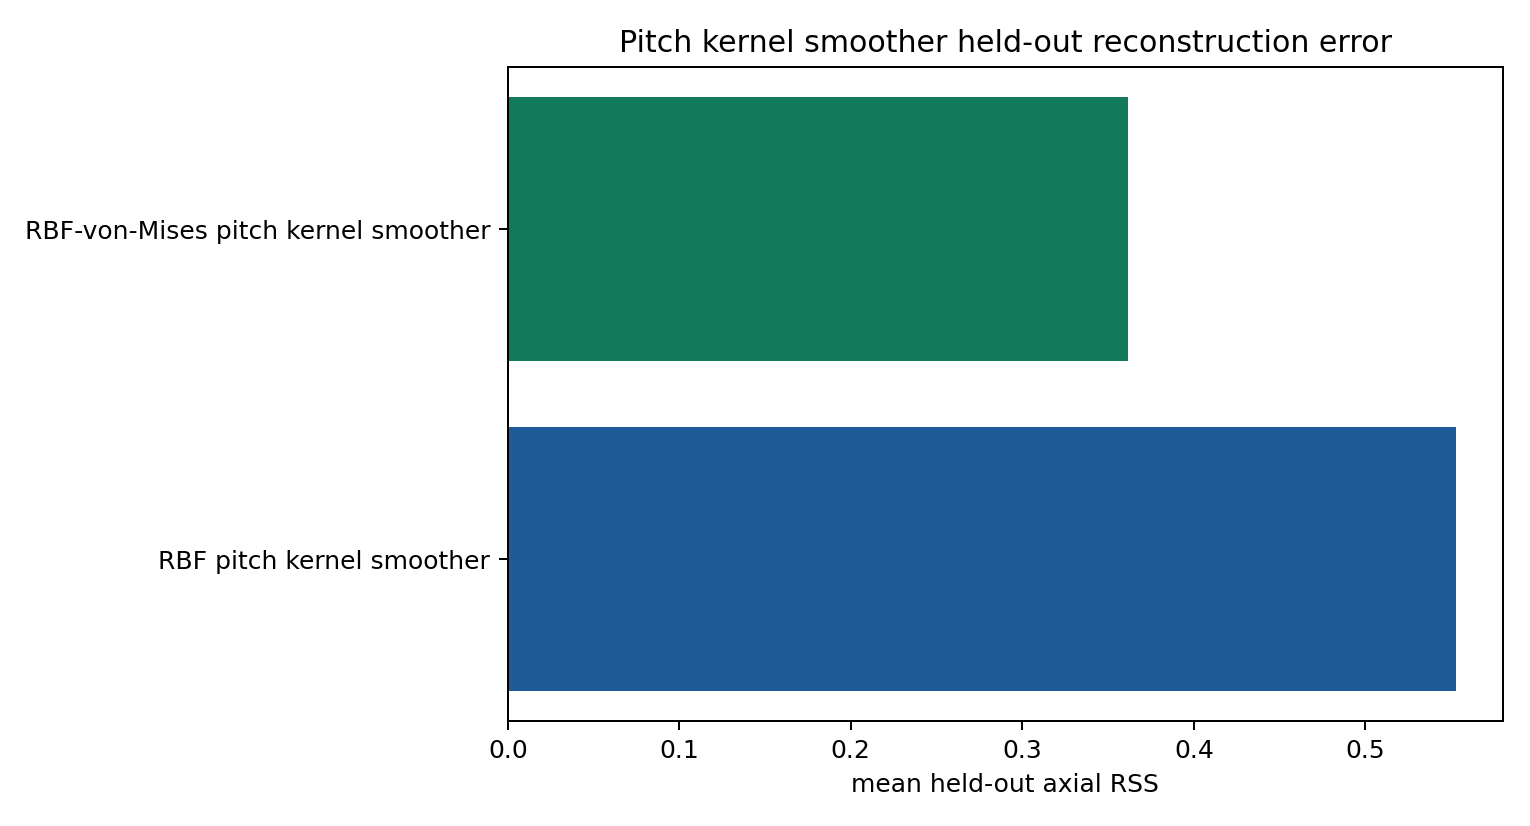
\includegraphics[width=0.78\linewidth]{plots/pitch_kernel_smoother_mean_rss.png}
\caption{Mean held-out axial RSS for the two pitch-kernel smoothers.}
\end{figure}

\begin{figure}[h!]
\centering
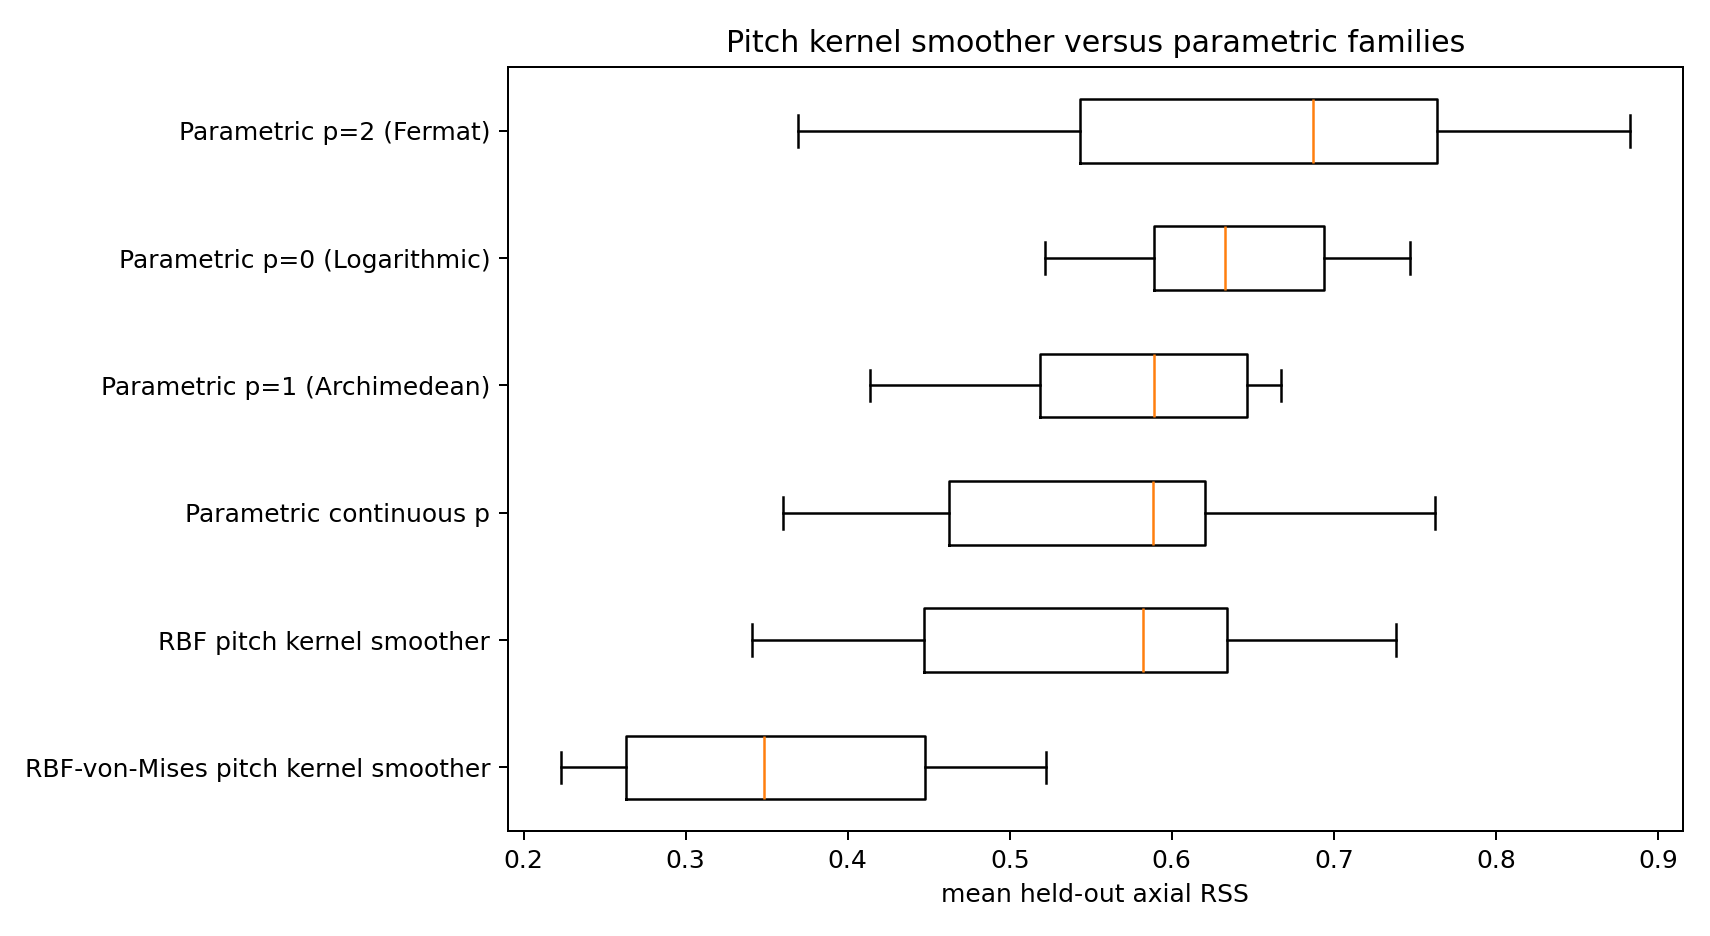
\includegraphics[width=0.86\linewidth]{plots/pitch_kernel_vs_parametric_boxplot.png}
\caption{Held-out axial RSS distribution comparing selected pitch-kernel smoothers with parametric families.}
\end{figure}

\FloatBarrier
\section{Streamline Overlays}
\begin{figure}[p]
\centering
\includegraphics[width=0.96\linewidth]{plots/streamline\_overlays/Front\_EE-1\_1\_3000x\_rings\_coords\_pitch\_kernel\_streamlines.png}
\caption{Notebook-style pitch-kernel and parametric streamline overlays for \texttt{Front\_EE-1\_1\_3000x\_rings\_coords.csv}. Observed Gabor arrows are shown at opacity $\alpha=0.7$.}
\end{figure}
\begin{figure}[p]
\centering
\includegraphics[width=0.96\linewidth]{plots/streamline\_overlays/Front\_EE-1\_2\_3000x\_rings\_coords\_pitch\_kernel\_streamlines.png}
\caption{Notebook-style pitch-kernel and parametric streamline overlays for \texttt{Front\_EE-1\_2\_3000x\_rings\_coords.csv}. Observed Gabor arrows are shown at opacity $\alpha=0.7$.}
\end{figure}
\begin{figure}[p]
\centering
\includegraphics[width=0.96\linewidth]{plots/streamline\_overlays/Front\_EE-1\_3\_3000x\_rings\_coords\_pitch\_kernel\_streamlines.png}
\caption{Notebook-style pitch-kernel and parametric streamline overlays for \texttt{Front\_EE-1\_3\_3000x\_rings\_coords.csv}. Observed Gabor arrows are shown at opacity $\alpha=0.7$.}
\end{figure}
\begin{figure}[p]
\centering
\includegraphics[width=0.96\linewidth]{plots/streamline\_overlays/Front\_EE-1\_4\_3000x\_rings\_coords\_pitch\_kernel\_streamlines.png}
\caption{Notebook-style pitch-kernel and parametric streamline overlays for \texttt{Front\_EE-1\_4\_3000x\_rings\_coords.csv}. Observed Gabor arrows are shown at opacity $\alpha=0.7$.}
\end{figure}
\begin{figure}[p]
\centering
\includegraphics[width=0.96\linewidth]{plots/streamline\_overlays/Front\_EE-1\_5\_3000x\_rings\_coords\_pitch\_kernel\_streamlines.png}
\caption{Notebook-style pitch-kernel and parametric streamline overlays for \texttt{Front\_EE-1\_5\_3000x\_rings\_coords.csv}. Observed Gabor arrows are shown at opacity $\alpha=0.7$.}
\end{figure}
\begin{figure}[p]
\centering
\includegraphics[width=0.96\linewidth]{plots/streamline\_overlays/Front\_EE1\_1\_3000x\_rings\_coords\_pitch\_kernel\_streamlines.png}
\caption{Notebook-style pitch-kernel and parametric streamline overlays for \texttt{Front\_EE1\_1\_3000x\_rings\_coords.csv}. Observed Gabor arrows are shown at opacity $\alpha=0.7$.}
\end{figure}
\begin{figure}[p]
\centering
\includegraphics[width=0.96\linewidth]{plots/streamline\_overlays/Front\_EE1\_2\_3000x\_rings\_coords\_pitch\_kernel\_streamlines.png}
\caption{Notebook-style pitch-kernel and parametric streamline overlays for \texttt{Front\_EE1\_2\_3000x\_rings\_coords.csv}. Observed Gabor arrows are shown at opacity $\alpha=0.7$.}
\end{figure}
\begin{figure}[p]
\centering
\includegraphics[width=0.96\linewidth]{plots/streamline\_overlays/Front\_EE1\_3\_3000x\_rings\_coords\_pitch\_kernel\_streamlines.png}
\caption{Notebook-style pitch-kernel and parametric streamline overlays for \texttt{Front\_EE1\_3\_3000x\_rings\_coords.csv}. Observed Gabor arrows are shown at opacity $\alpha=0.7$.}
\end{figure}
\begin{figure}[p]
\centering
\includegraphics[width=0.96\linewidth]{plots/streamline\_overlays/Front\_EE1\_4\_3000x\_rings\_coords\_pitch\_kernel\_streamlines.png}
\caption{Notebook-style pitch-kernel and parametric streamline overlays for \texttt{Front\_EE1\_4\_3000x\_rings\_coords.csv}. Observed Gabor arrows are shown at opacity $\alpha=0.7$.}
\end{figure}
\begin{figure}[p]
\centering
\includegraphics[width=0.96\linewidth]{plots/streamline\_overlays/Front\_EE1\_5\_3000x\_rings\_coords\_pitch\_kernel\_streamlines.png}
\caption{Notebook-style pitch-kernel and parametric streamline overlays for \texttt{Front\_EE1\_5\_3000x\_rings\_coords.csv}. Observed Gabor arrows are shown at opacity $\alpha=0.7$.}
\end{figure}

\end{document}
